\documentclass[preview]{standalone}

\usepackage{amsmath}
\usepackage{amssymb}
\usepackage{tikz}
\usepackage{pgfplots}
\usepackage{wrapfig}
\usepackage{stellar}
\usepackage{definitions}
\usepackage{bettelini}
\usepackage{xfrac}

\usetikzlibrary{positioning, arrows.meta}

\begin{document}

\id{definite-integrals}
\genpage

\section{Step functions}

\begin{snippetdefinition}{indicator-function-definition}{Indicator function}
    Let \(A\) be a \set.
    The \textit{indicator function} of \(A\) is defined as
    \[
        1_{A}(x) \triangleq \begin{cases}
            1 & x \in A \\
            0 & x \notin A
        \end{cases}
    \]
\end{snippetdefinition}

\begin{snippetdefinition}{function-positive-part-definition}{Function positive part}
    Let \(f(x)\) be a real-valued \function.
    The \emph{positive part} of \(f(x)\) is defined as
    \[
        f^+(x) = \max\{f(x), 0\}
    \]
\end{snippetdefinition}

\begin{snippetdefinition}{function-negative-part-definition}{Function negative part}
    Let \(f(x)\) be a real-valued \function.
    The \emph{negative part} of \(f(x)\) is defined as
    \[
        f^-(x) = -\min\{f(x), 0\}
    \]
\end{snippetdefinition}

\begin{snippetproposition}{positive-negative-part-property}{}
    Let \(f(x)\) be a real-valued \function. Then,
    \[
        f^+ = \frac{|f| + f}{2}, \qquad
        f^- = \frac{|f| - f}{2}
    \]
\end{snippetproposition}

\begin{snippetdefinition}{step-function-definition}{Step function}
    Let \(f\colon \realnumbers \fromto \realnumbers\) be a \function. Then, \(f\) is a \emph{step function}
    if it can be wrriten as
    \[
        f(x) = \sum_{i=0}^n \alpha_i \indicator_{A_i}(x)
    \]
    where \(\alpha_i\in\realnumbers\) and \(A_i\) are intervals.
\end{snippetdefinition}

\begin{snippetdefinition}{dirichlet-function-definition}{Dirichlet function}
    The \emph{Dirichlet function} is defined as \(\indicator_{\rationalnumbers}\).
\end{snippetdefinition}

\begin{snippetdefinition}{riemann-integral-definition}{Riemann integral}
\end{snippetdefinition}

\section{Definite integrals}

\begin{snippet}{area-problem-illustration}
    \begin{wrapfigure}{l}{10cm}
        \begin{center}
            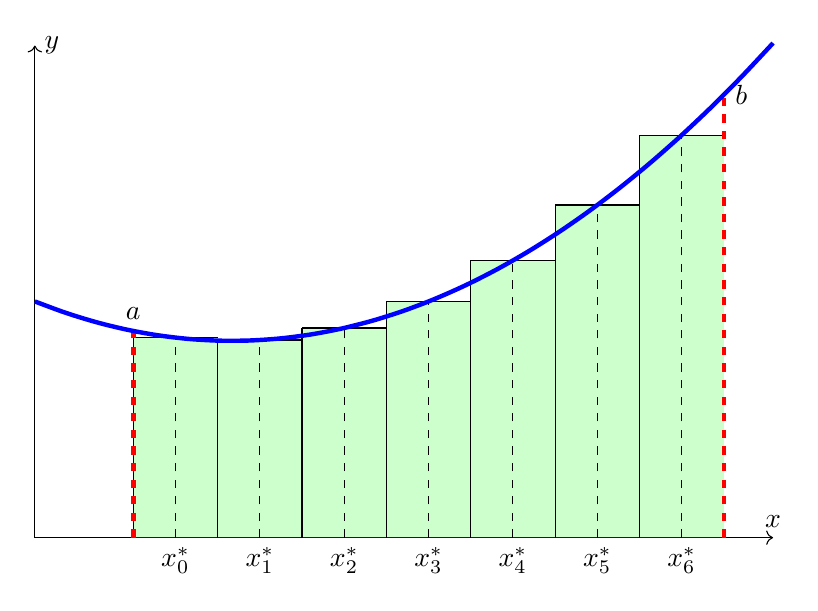
\begin{tikzpicture}[
                scale=1.25,
                declare function={
                    func(\x) = 0.1 * (\x - 2) * (\x - 2) + 2;
                    Width=7.5;
                    Height=5;
                    A = 1;
                    B = 7;
                    N = 7;
                    Delta = {(B-A) / N};
                }
            ]
                \draw[->] (0, 0) -- (0, Height) node[right] {\(y\)};
                \draw[->] (0, 0) -- (Width, 0) node[above] {\(x\)};
        
                \pgfmathtruncatemacro\END{N-1}
                \foreach \x in {0,1,...,\END} {
                    % rectangle
                    \fill [green, opacity=0.2]
                        ({A + Delta * \x}, 0) rectangle ({A + Delta * (\x+1)}, {func(A + Delta * (\x + 0.5))});
                    
                    \draw[-] ({A + Delta * \x}, 0)
                        -- ({A + Delta * \x}, {func(A + Delta * (\x + 0.5))});

                    \draw[-, dashed] ({A + Delta * (\x + 0.5)}, 0)
                        node[below] {\(x_{\x}^*\)}
                        -- ({A + Delta * (\x + 0.5)}, {func(A + Delta * (\x + 0.5))});

                    % line over rectangle
                    \draw[-] ({A + Delta * \x}, {func(A + Delta * (\x + 0.5))})
                        -- ({A + Delta * (\x+1)}, {func(A + Delta * (\x + 0.5))});
                }
        
                \draw[-, dashed, red, ultra thick] (A, 0) -- (A, {func(A)}) node[above, black] {\(a\)};
                \draw[-, dashed, red, ultra thick] (B, 0) -- (B, {func(B)}) node[right, black] {\(b\)};
        
                \draw[domain=0:Width, smooth, variable=\x, blue, ultra thick] plot ({\x}, {func(\x)});
            \end{tikzpicture}
        \end{center}
    \end{wrapfigure}

    We want to find the signed area between \(f(x)\) and the \(x\)-axis between
    the interval \([a;b]\).\\
    One way to do it would be by dividing the area into \(n\) rectangles, each of width
    \[
        \Delta x = \frac{b-a}{n}
    \]
    The height of each triangle is given by \(f(x_k^*)\).
    The area under the curve is approximately
    \[
        A \approx \sum_{k=0}^{n-1}f(x_k^*)\Delta x
    \]
    Notice that the position of \(x_k^*\) within the base of each rectangle controls the type of
    the approximation of the area under the curve.
    By moving \(x_k^*\) within the base we may achieve an approximation by abundance
    or defect.
    The type of approximation does not matter when we let \(n\to \infty\).
    As the amount of rectangles approaches infinity, the approximation approaches
    the exact value of the area.
    \[
        A = \lim_{n\to\infty} \sum_{k=0}^{n}f(x_k^*)\Delta x
    \]
    \wrapfill
\end{snippet}

\begin{snippetproposition}{definite-integral-inversion}{}
    \[
        \integral[a][b][f(x)][x] = -\integral[b][a][f(x)][x]
    \]
\end{snippetproposition}

\subsection{Fundamental Theorem of Calculus}

\begin{snippettheorem}{fundamental-theorem-of-calculus}{Fundamental Theorem of Calculus}
    A primitive function \(F(x)\) such that \(F(0)=0\) represents the signed area
    from \(0\) to \(x\) of \(f(x)\). \\
    Let \(f(x)\) be continuous on the interval \(I=[a;b]\) and \(F(x)\) any \primitivefunc of \(f(x)\),
    then \(F(x)\) is also continuous on \(I\) and
    \[
        \integral[0][x][f(t)][t] = F(x)
    \]
    and
    \[
        \integral[a][b][f(x)][x] = F(b) - F(a)
    \]
    This also means that
    \[
        f(x)=\integral[0][x][f'(t)][t]
    \]
    or
    \[
        \frac{d}{dx}\integral[a][x][f(t)][t]=f(x)
    \]
\end{snippettheorem}

\begin{snippetcorollary}{fundamental-calculus-theorem-corollary-1}{Non-constant integral limits derivative}
    When the upper or lower limit is not constant,
    \begin{align*}
        \frac{d}{dx} \integral[v(x)][u(x)][f(t)][t]
        &= \frac{d}{dx} \left[ F(u(x)) - F(v(x)) \right] \\
        &= u'(x)f(u(x)) - v'(x)f(v(x))
    \end{align*}
\end{snippetcorollary}

\section{Average Function Value}

\begin{snippettheorem}{average-function-value}{Average Function Value}
    The average value of a continuous function \(f(x)\) over the interval \([a;b]\) is given by
    \[
        f_\text{avg} = \frac{1}{b-a} \integral[a][b][f(x)][x]
    \]
\end{snippettheorem}

\section{Mean Value Theorem}

\begin{snippettheorem}{mean-value-theorem}{Mean Value Theorem}
    If \(f(x)\) is a continuous function on \(I=[a;b]\), \(f(x)\) will at some point in \(I\)
    reach its average value, meaning
    \[
        \exists c \suchthat f(c) = \frac{1}{b-a} \integral[a][b][f(x)][x]
    \]
\end{snippettheorem}

\section{Area Between Functions}

\begin{snippet}{area-between-functions-illustration}
    \begin{wrapfigure}{l}{7.5cm}
        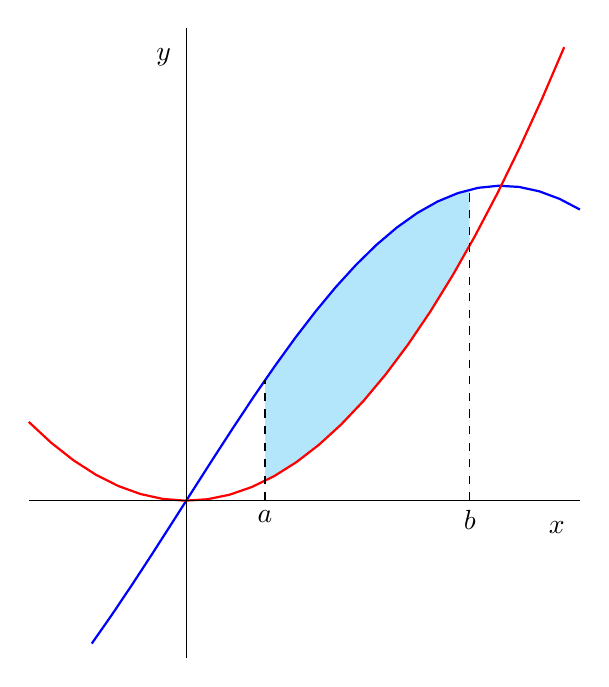
\begin{tikzpicture}[x=4cm, y=4cm, >=Stealth, declare function={
            func1(\x) = sin(3.14*\x/2 r);
            func2(\x) = \x*\x;
            a=0.25;
            b=0.9;
        }]
            % area under func1 
            \fill[cyan!30!white] plot[domain=a:b] (\x,{func1(\x)}) -- plot[domain=b:a] (\x,{0}) -- cycle;
            

            % area under func2
            \fill[white] plot[domain=a:b] (\x,{func2(\x)}) -- plot[domain=b:a] (\x,{0}) -- cycle;
            
            % func1
            \draw[blue, -, thick] plot[domain=-0.3:1.25] (\x,{func1(\x)});
            
            % func2
            \draw[red, -, thick]  plot[domain=-0.5:1.2] (\x,{func2(\x)});

            \draw[-, dashed] (a, 0) node[below] {\(a\)} -- (a, {func1(a)});
            \draw[-, dashed] (b, 0) node[below] {\(b\)} -- (b, {func1(b)});

            \draw[-] (-.5,0) -- (1.25, 0)
                node[below left=4pt and 2pt] {\(x\)};
            \draw[-] (0,-.5) -- (0,1.5)
                node[below left=4pt and 2pt] {\(y\)};
        \end{tikzpicture} 
    \end{wrapfigure}

    Given a \function \(y=f(x)\) and \(y=g(x)\), the area enclosed by the two functions
    in the interval \(I=[a;b]\) is given by
    \[
        A=\integral[a][b][f(x)-g(x)][x]
    \]
    assuming that \(f(x)\geq g(x)\) when \(x\in I\). \\
    Note that \(A\geq 0\). \\
    If \(f(x)<g(x)\) for some \(x\in I\) this formula won't work. However, it is still
    possible to split the integral into multiple integrals at every point where \(f(x) - g(x)\) changes sign.
    To remove the sign contraint we could say
    \[
        A = \integral[a][b][|f(x)-g(x)|][x]
    \]
    \wrapfill
    \vspace{-2.5cm}
    \begin{wrapfigure}{l}{7.5cm}
        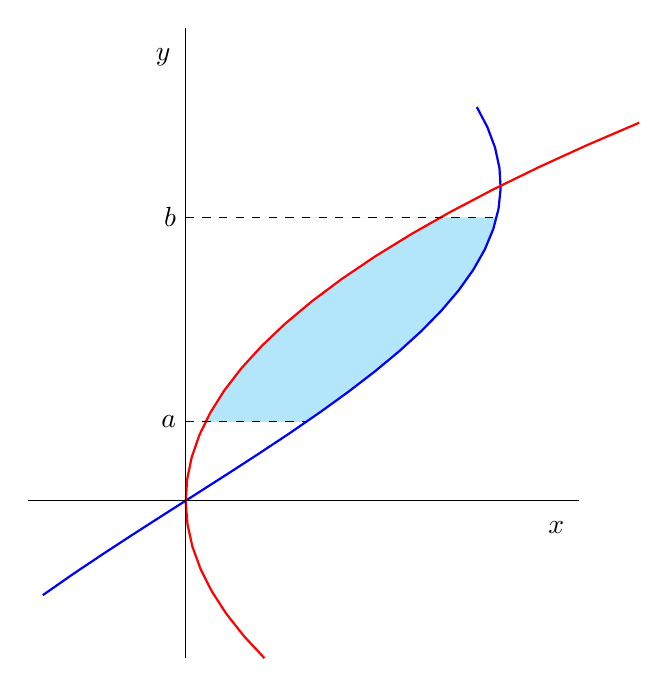
\begin{tikzpicture}[x=4cm, y=4cm, >=Stealth, declare function={
            func1(\x) = sin(3.14*\x/2 r);
            func2(\x) = \x*\x;
            a=0.25;
            b=0.9;
        }]
            % area under func1 
            \fill[cyan!30!white] plot[domain=a:b] ({func1(\x)},\x) -- plot[domain=b:a] ({0}, \x) -- cycle;
            

            % area under func2
            \fill[white] plot[domain=a:b] ({func2(\x)}, \x) -- plot[domain=b:a] ({0}, \x) -- cycle;
            
            % func1
            \draw[blue, -, thick] plot[domain=-0.3:1.25] ({func1(\x)}, \x);
            
            % func2
            \draw[red, -, thick]  plot[domain=-0.5:1.2] ({func2(\x)}, \x);

            \draw[-, dashed] (0, a) node[left] {\(a\)} -- ({func1(a)}, a);
            \draw[-, dashed] (0, b) node[left] {\(b\)} -- ({func1(b)}, b);

            \draw[-] (-.5,0) -- (1.25, 0)
                node[below left=4pt and 2pt] {\(x\)};
            \draw[-] (0,-.5) -- (0,1.5)
                node[below left=4pt and 2pt] {\(y\)};
        \end{tikzpicture} 
    \end{wrapfigure}

    The same thing applies when we have functions in the form \(x=f(y)\) and \(x=g(y)\)
    and we want to find the areas enclosed by the functions when \(y\in [d;c]\)
    \[
        A=\integral[d][c][|f(y)-g(y)|][y]
    \]
    \wrapfill
    \vspace{-2.5cm}
\end{snippet}

\begin{snippetproof}{area-of-circle-theorem-proof}{area-of-circle-theorem}{}
    The equation for a circle is \(x^2 + y^2 = r^2\).
    To compute its area, we can consider the function of the upper semicircle
    and compute the area from \(0\) to \(r\). This will prove the area
    of a quarter of the circle. Thus, the full area is given by
    \[
        4\integral[0][r][\sqrt{r^2 - x^2}][x]
    \]
    We substitute \(x = r\sin\theta\), meaning \(dx = r\cos\theta\,d\theta\).
    Note that when \(x=0\), \(\theta = 0\) and when \(x=r\), \(\theta = \picircle / 2\).
    \begin{align*}
        4\integral[0][r][\sqrt{r^2 - x^2}][x]
        &= 4\integral[0][\picircle / 2][\sqrt{r^2 - r^2\sin^2\theta}r\cos\theta][u] \\
        &= 4\integral[0][\picircle / 2][r^2\cos\theta \sqrt{1-\sin^2\theta}][u] \\
        &= 4r^2\integral[0][\picircle / 2][\cos^2\theta][u] \\
        &= 4r^2\integral[0][\picircle / 2][\frac{1 + \cos(2\theta)}{2}][u] = r^2\picircle
    \end{align*}
\end{snippetproof}

\end{document}